\subsection{Công nghệ front-end}
\subsubsection{ReactJS}
\paragraph{Khái quát về ReactJS}

Ngày nay ReactJS đã trở nên rất phổ biến bởi những tính năng
linh hoạt và đơn giản với hơn 1.300.000 developer và hơn 94.000
trang web đang sử dụng ReactJS
(theo số liệu thống kê trên blog topdev.vn). 
ReactJS là một thư viện JavaScript mã nguồn mở được thiết kế
bởi Facebook để tạo ra những ứng dụng web hấp dẫn, nhanh và
hiệu quả với source code tối thiểu. Mục đích cốt lõi của
ReactJS không chỉ khiến cho trang web phải thật mượt mà còn
phải nhanh, khả năng mở rộng cao và đơn giản. Trên website chính
thức của React tổng quan rằng: ReactJS –
“A JavaScript for library for building user interface”,
tức là React sinh ra để phục vụ tầng View,
tập trung vào xây dựng giao diện. 

Tư tưởng của ReactJS là xây dựng lên các component có
tính tái sử dụng, dễ dàng cho việc chia nhỏ vấn đề, kiểm thử,
giúp chúng ta dễ dàng quản lý, mở rộng hệ thống. Đặc tính của
ReactJS là luôn giữ các component ở trạng thái stateless nhiều
nhất có thể, khiến ta dễ dàng quản lý nó. Bản thân các component
này không có trạng thái, nó nhận đầu vào từ bên ngoài và
chỉ hiển thị ra dựa vào các đầu vào đó, điều này
cũng lý giải tính tái sử dụng (reuse) và tiện lợi
trong kiểm thử (testing) của ReactJS.

\paragraph{Virtual DOM}
Sử dụng ReactJS, ta thường hay nghe tới Virtual DOM,
DOM thì rất quen thuộc với những lập trình viên front-end,
còn Virtual DOM là gì? Có khác gì với DOM không? 

\begin{figure}[H]
\centering
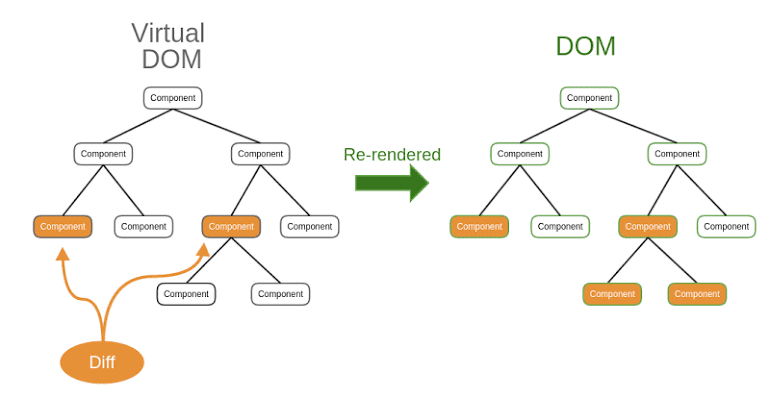
\includegraphics[width=10cm]{images/DOM.png}
\caption{Kiến trúc của DOM}
\label{fig:dom}
\end{figure}

Trước tiên, DOM là viết tắt của Document Object Model là
một chuẩn được định nghĩa bởi W3C dùng để truy xuất và thao
tác trên code HTML bằng các ngôn ngữ lập trình thông dịch
(scripting language) như JavaScript.
Trong Hình \ref{fig:dom}
trên có thể thấy tất cả các thẻ HTML sẽ được quản lý trong
các đối tượng document, thẻ cao nhất là thẻ html, tiếp đến là
phân nhánh body và head, trong head có thẻ style, title, … trong body
chứa các thẻ html. Như vậy thông qua DOM, JavaScript có thể thay
đổi tất cả các phần tử HTML, các thuộc tính HTML, CSS, loại
bỏ hoặc thêm các thành phần và thuộc tính HTML mới, tạo ra các sự
kiện khi tương tác,… Tức là bạn có thể thay đổi cả trang web với DOM.

Khi DOM thay đổi, trình duyệt phải tính toán lại CSS và dựng lại
trang web, điều này sẽ tốn thời gian, nhất là với những ứng dụng
Single Page Application, việc sửa đổi DOM là liên tục không ngừng
nghỉ. Hay khi xử lý các sự kiện (event) như click, submit, …
DOM sẽ tìm tất cả các node liên quan đến sự kiện và cập nhật nếu
thấy nó cần thiết. Vậy thì có cần thiết khi phải tìm tất
cả các node liên quan không? Hay sẽ hiệu quả hơn khi chỉ tìm
node nào cần cập nhật.

Virtual DOM xuất hiện để giải quyết những vấn đề này.
Virtual DOM gắn với ReactJS, thay vì xử lý DOM Tree thủ công,
chúng định nghĩa các component trông giống DOM
(vì vậy mà cú pháp JSX nhìn rất giống HTML), còn ReactJS sẽ thực
hiện công việc ở tầng thấp hơn. Tổng quát thì Virtual DOM là
một định dạng dữ liệu JavaScript nhẹ dùng để thể hiện nội dung
của DOM tại một thời điểm nhất định nào đó. Nó có tất cả các thuộc
tính giống như DOM nhưng không có khả năng tương tác lên màn hình như
DOM. Sự đặc biệt của Virtual DOM nằm ở cơ chế Snapshots và Diffing.
Khi cần cập nhật phần tử giao diện, React sẽ lấy một snapshot của Virtual
DOM (có thể hiểu là bản ghi trạng thái ngay lúc đó),
sử dụng snapshot này để so sánh với một Virtual DOM trước
khi thực hiện thay đổi.

\begin{figure}[H]
\centering
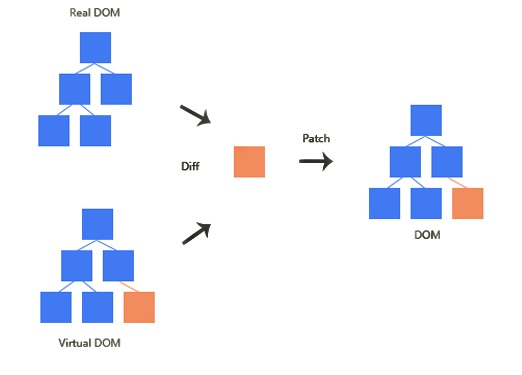
\includegraphics[width=12cm]{images/virtualdom.jpg}
\caption{Virtual DOM Snapshots \& Diffing}
\label{fig:virtualdom}
\end{figure}

\paragraph{Single Page Application (SPA)}
Với ReactJS, ta dễ dàng tạo ra một Single Page Application (SPA).
Khác với những ứng dụng web truyền thống, Single Page Application
có một trang gốc và trong trang gốc đó, chúng ta có thể tải
nhiều trang con (tương ứng với các thành phần của trang gốc) mà
không gây bất kì ảnh hưởng gì đến trang gốc. Trong khi các
ứng dụng web truyền thống phải tải lại toàn bộ trang khi
chúng ta tương tác với trang web thì Single Page Application chỉ load
phần trang cần thiết. Các thành phần chung như header, footer, menu,
side bar,… thường xuất hiện ở nhiều trang của ứng dụng sẽ được
Single Page Application load một lần duy nhất ở trang gốc.

\begin{figure}[H]
\centering
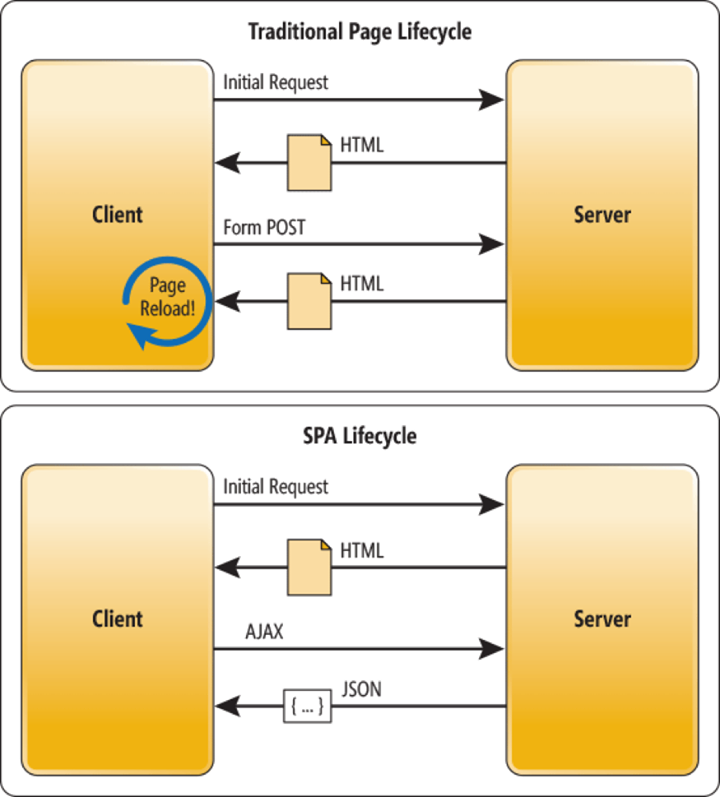
\includegraphics[width=11cm]{images/spa.png}
\caption{Single Page Application }
\label{fig:spa}
\end{figure}

Do vậy Single Page Application mang lại nhiều ưu điểm như:
\begin{itemize}[topsep=0ex]
\item Thứ nhất, việc render HTML ở server sẽ cực kì tốn
    tài nguyên nếu trang web có nhiều người dùng, với Single Page
    Application điều này chỉ xảy ra lần đầu tiên khi người dùng
    truy cập trang chủ (hoặc có thể không cần render trên server),
    còn sau đó việc render sẽ do client đảm nhiệm. 

\item Thứ hai, Single Page Application tách biệt front-end và
    back-end, SPA giao tiếp với server chủ yếu qua JSON REST API
    giúp cho dữ liệu gửi và trả giữa client và server giảm
    đến mức tối thiểu. Việc phát triển, kiểm thử cũng có thể
    độc lập giữa front-end và back-end. 

\item Thứ ba, trong suốt quá trình sử dụng, chỉ có dữ liệu là
    được truyền qua lại giữa client và server, còn các tài
    nguyên tĩnh (HTML, CSS, Script, …) chỉ được tải một
    lần duy nhất, vì vậy sẽ giảm thiểu băng thông cho server. 

\item Thứ tư, Single Page Application giúp tăng trải nghiệm người
    dùng, là một ứng dụng web nhưng người dùng tương tác
    giống như một ứng dụng cho Desktop vậy.
\end{itemize}

\paragraph{React Router}
React Router là thư viện định tuyến (routing) chuẩn của React,
nó giúp giao diện của ứng dụng đồng bộ với URL trên trình duyệt.
React Router cho phép định tuyến luồng dữ liệu (data-flow) trong
ứng dụng web một cách rõ ràng. Với React Router, việc xây dựng
Single Page Application trở nên vô cùng dễ dàng.

\begin{figure}[H]
\centering
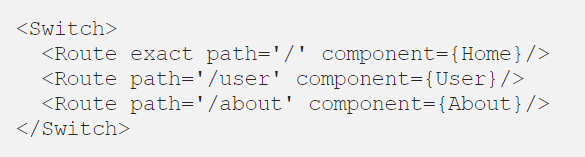
\includegraphics[width=11cm]{images/react-router.png}
\caption{Ví dụ React Router}
\label{fig:reactrouter}
\end{figure}

Hình \ref{fig:reactrouter} trên thể hiện cấu hình 
cơ bản của React Router với
đường dẫn (/path) và Route và giao diện tương ứng.

\subsubsection{Redux}
\paragraph{Khái quát về Redux}
Một ứng dụng web sẽ nhận dữ liệu từ phía máy chủ (back-end),
hay nhận những thao tác của người dùng (input, click, submit, …),
những thứ này chúng ta gọi đó là trạng thái (state) của ứng dụng.
Nếu biết được trạng thái của ứng dụng tại một thời điểm nào đó,
chúng ta sẽ biết vào thời điểm đó ứng dụng đã nhận dữ liệu nào,
những thao tác nào đã được người dùng truyền lên.

Ví dụ: Khi chúng ta click vào nút Back / Forward trên trình duyệt 
thì mỗi trang là một trạng thái của ứng dụng.

Như đã trình bày ở trên, ReactJS xây dựng lên các Single
Page Application, tức chỉ render một trang, và tất cả các
thành phần của ứng dụng sẽ được lưu trữ trong đó. Vì thế,
nếu ứng dụng phức tạp lên theo thời gian, các component sẽ nhiều
lên, và việc quản lý các state của chúng cũng ngày một lớn dần.
Giao diện ứng dụng (UI) cũng trở nên phức tạp vì chúng ta
cần quản lý các công việc active Routes, selected tabs, spinners,
pagination, … Trong ReactJS để truyền dữ liệu giữa các component anh
em, một state phải tồn tại (live) trong một component cha,
một phương thức (method) để update chính state này được cung cung
cấp bởi component cha, từ đây sẽ truyền xuống props của các
component con. Do vậy nếu một state phải được chia sẻ giữa các
component cách khá xa nhau trong một tree component thì state
này sẽ phải được truyền từ một component đến một component khác cho
đến khi nó đến được nơi mà nó được gọi.

\begin{figure}[H]
\centering
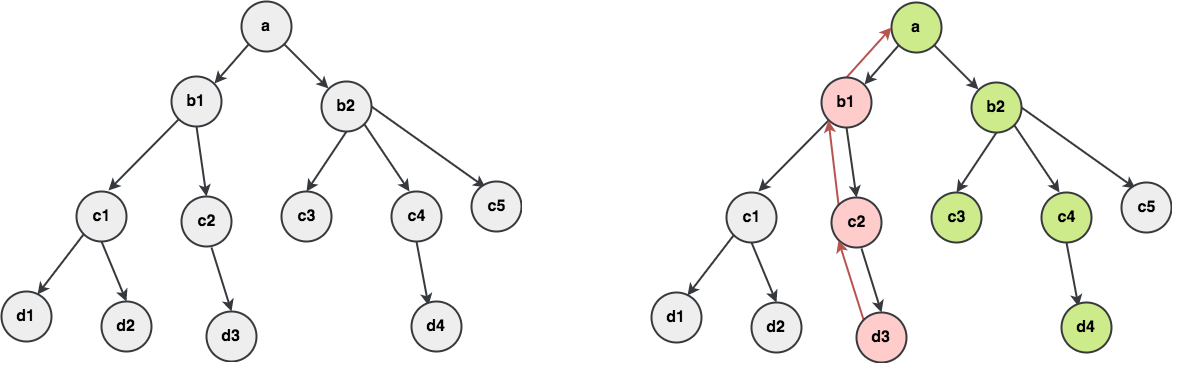
\includegraphics[width=16cm]{images/redux-state-transfer.png}
\caption{Truyền state giữa các component}
\end{figure}

Trong hình vẽ trên, giả sử nếu có một sự kiện ở node d3 kích
hoạt muốn thay đổi state d4 thì luồng dữ liệu sẽ được truyền
từ node d3 trở về node gốc là a, sau đó từ node a lại truyền data
đến các node con. Thứ tự truyền: d3 – c2 – b1 – a – b2 – c4 – d4.
Tương tự nếu muốn thay đổi state ở c3 thì thứ tự truyền là:
d3 – c2 – b1 – a – b2 – c3. Điều này làm cho bộ phận quản lý
state trong ứng dụng trở nên phức tạp và bừa bộn, do vậy ta
cần một công cụ quản lý trạng thái (state management tool)
như Redux. Giải pháp Redux đưa ra như sau:

\begin{figure}[H]
\centering
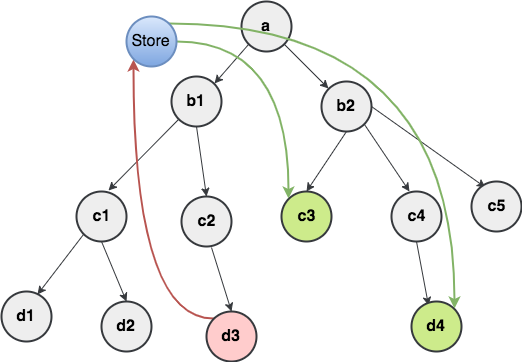
\includegraphics[width=10cm]{images/redux-solution.png}
\caption{Quản lý state trong Redux}
\end{figure}

Quay lại ví dụ ở trên thì ta cần map sự kiện từ node d3
về store của Redux rồi ở node d4, c3 cần connect với store
và cập nhật dữ liệu thay đổi.

\paragraph{Nguyên lý vận hành của Redux}
Cách Redux hoạt động khá đơn giản. Redux có một store lưu trữ
toàn bộ state của ứng dụng. Mỗi component có thể truy cập trực
tiếp đến state được lưu trữ thay vì phải truyền từ component
này qua component khác.

\begin{figure}[H]
\centering
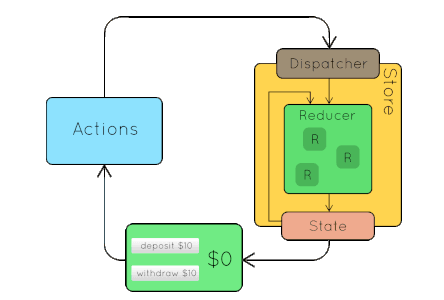
\includegraphics[width=12cm]{images/redux-without-middleware.png}
\caption{Kiến trúc của Redux}
\end{figure}

Redux có 3 thành phần là Action, Store và Reducer.

Action đơn giản là các sự kiện, mô tả những gì xảy ra như 
là cách mà chúng ta gửi dữ liệu từ ứng dụng đến Redux store, 
dữ liệu có thể đến từ sự tương tác của user và ứng dụng, 
API call hoặc khi submit một form, … Tuy nhiên action lại không 
chỉ rõ phần state nào thay đổi, việc này do Reducer đảm nhiệm. 
Reducer nhận vào một state cũ và action được gửi lên 
sau đó trả về một state mới. 

\begin{lstlisting}
(previousState, action) => newState
\end{lstlisting}

Những state này được lưu như những đối tượng (objects) và
chúng định rõ cách state của một ứng dụng thay đổi trong việc
phản hồi một action gửi đến store. Store là nơi lưu lại các
state của ứng dụng và nó là duy nhất
trong bất kì một ứng dụng Redux nào.

\paragraph{Middleware}
Một ứng dụng thực tế đòi hỏi có những thao tác xử lý cần thời
gian để phản hồi (các thao tác bất đồng bộ lấy dữ liệu từ
api hay các thao tác đọc ghi file hay đọc cookie từ trình duyệt, …),
các thao tác như vậy gọi là side effect. Để giải quyết được
các side effect này, trong Redux ta cần thực hiện nó ở middleware.

Trong Redux, Middleware cho phép chúng ta can thiệp vào giữa
thời điểm dispatch một action và thời điểm action đó đến được
reducer. Kiến trúc của Redux đầy đủ khi có middleware như hình dưới đây.

\begin{figure}[H]
\centering
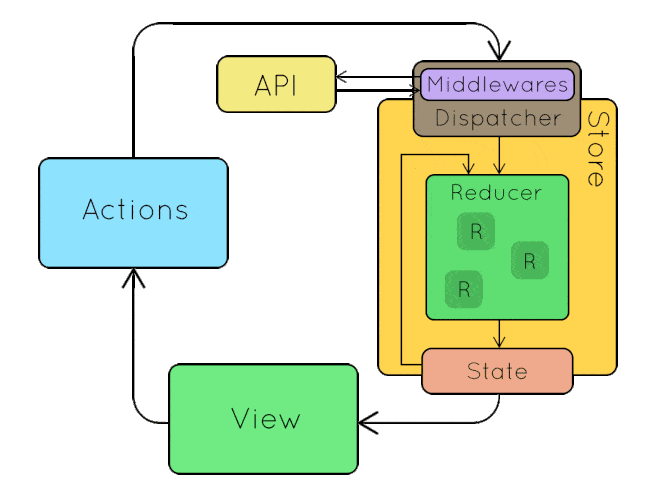
\includegraphics[width=12cm]{images/redux-architecture.png}
\caption{Kiến trúc của Redux với Middleware}
\end{figure}

Ta có thể tự viết một middleware hoặc có thể dùng những thư
viện middleware được xây dựng sẵn. Hiện tại có một vài thư viện
middleware cho Redux, ví dụ như redux-thunk, redux-saga,
redux-observable, … mỗi thư viện có phương pháp giải quyết
vấn đề side-effect riêng.
Trong project này sử dụng redux-saga để xử lý các side-effect.

\paragraph{Redux-saga}
Redux-saga là một thư viện hỗ trợ việc xử lý side-effect trong
ứng dụng React/Redux (ví dụ như xử lý bất đồng bộ khi load dữ liệu,…)
và làm cho các ứng dụng này trở nên đơn giản hơn.
Bằng cách sử dụng Generator Function, redux-saga giúp ta viết
code bất đồng bộ (async code) nhìn giống như là đồng bộ (synchronos).

Generator Function là function có khả năng hoãn lại quá trình
thực thi mà vẫn giữ nguyên được ngữ cảnh của function. Khác với
function bình thường là thực thi và trả về kết quả,
thì Generator function có thể thực thi, tạm dừng trả về
kết quả và thực thi tiếp (bằng cách sử dụng từ khóa \textbf{yield}).
Nếu như function bình thường khi được gọi sẽ thực thi hết tất cả
các câu lệnh trong hàm thì Generator function có khả năng tạm ngưng
trước khi hàm kết thúc và có thể tiếp tục chạy tại một thời điểm khác.
Chính chức năng này giúp ta giải quyết được vấn đề bất đồng bộ,
hàm sẽ dừng và đợi async chạy xong rồi tiếp tục thực thi.

\textit{Nguyên lý hoạt động của Redux-saga:} \\
Redux-saga cung cấp các hàm helper effect, các hàm này sẽ
trả về một effect object chứa các thông tin chỉ dẫn middleware
của Redux có thể thực hiện tiếp các hành động khác. Các hàm
helper effect sẽ được thực thi trong các generator function.
Ví dụ một số helper effect trong Redux-saga:
\begin{itemize}
\item \textit{takeEvery()}:
    thực thi và trả về kết quả của một action được gọi
\item \textit{takeLastest()}: nếu ta thực hiện một loạt các actions,
    nó sẽ chỉ thực thi và trả về kết quả của action cuối cùng.
\item \textit{put()}: dispatch một action.
\item \textit{call()}: gọi một function. Nếu nó trả về một Promise,
    sẽ tạm dừng saga cho đến khi Promise được giải quyết.
\end{itemize}
Ví dụ sử dụng helper effect trong Redux-saga:
\begin{lstlisting}[language=JavaScript,caption={Sử dụng Redux-Saga},captionpos=b]
// execute fetchPersonListSaga
// when action FETCH_PERSON_LIST is dispatched
yield takeEvery(FETCH_PERSON_LIST, fetchPersonListSaga);

// dispatch action pushSuccessNotification 
yield put(pushSuccessNotification(sequence, "Saved"));
\end{lstlisting}

% \subsubsection{Material-UI}
% \paragraph{Material Design}
% Material UI là một thư viện các React Component và được 
% tích hợp thêm cả Google’s Material Design. Trước tiên, 
% chúng ta sẽ tìm hiểu về nguyên lý Material Design. 

% Material Design là phong cách thiết kế áp dụng chủ yếu trong thiết
% kế ứng dụng Web, ứng dụng Mobile và đã trở thành một xu hướng
% phổ biến hiện nay. Đối với những Designer thiết kế UX/UI
% (giao diện / trải nghiệm người dùng), hay các lập trình viên
% front-end thì thuật ngữ Material Design không còn xa lạ.
% Có rất nhiều ứng dụng nổi tiếng thiết kế theo phong
% cách Material Design như các ứng dụng của Google
% (Google+, Gmail, Google Maps, …), Evernote, ePay, …

% \begin{figure}[H]
% \centering
% 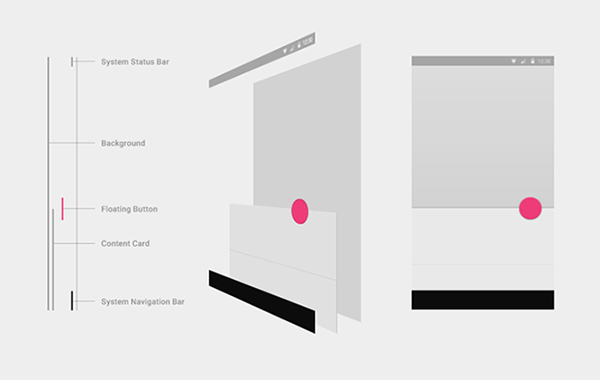
\includegraphics[width=14cm]{images/material-design.png}
% \caption{Thiết kế Material Design}
% \end{figure}

% Material Design là hình thức phát triển cao hơn của
% Flat Design (thiết kế phẳng), tuy nhiên thay vì cảm
% giác “phẳng lì” trên toàn bộ giao diện, Material Design là
% những lớp xếp chồng lên nhau, tạo chiều sâu, điểm nhấn hơn
% những thiết kế phẳng thông thường. Material Design chủ yếu tập
% trung vào những đường nét đơn giản, sử dụng những gam màu đậm,
% nổi bật, đồng thời cũng thường sử dụng những yếu tố đồ họa
% có cảm giác 3D, có hiệu ứng “nổi lên” (float) trên giao diện.
% Ngoài ra, thiết kế này còn bao gồm những chuyển động tự nhiên,
% tất cả những điều này đều nhằm mục đích mang lại cho người
% dùng trải nghiệm mới mẻ, thú vị và gần gũi hơn.

% Material Design có 3 yếu tố căn bản:
% \begin{itemize}[topsep=0ex]
% \item Thứ nhất là không gian: 
%     Không gian dưới lớp kính màn hình thiết bị được mô phỏng
%     như một không gian 3 chiều Oxyz với chiều sâu là trục Oz.
%     Để tạo chiều sâu cho thiết kế, designer cần điều chỉnh ánh
%     sáng một cách phù hợp.

% \begin{figure}[H]
% \centering
% 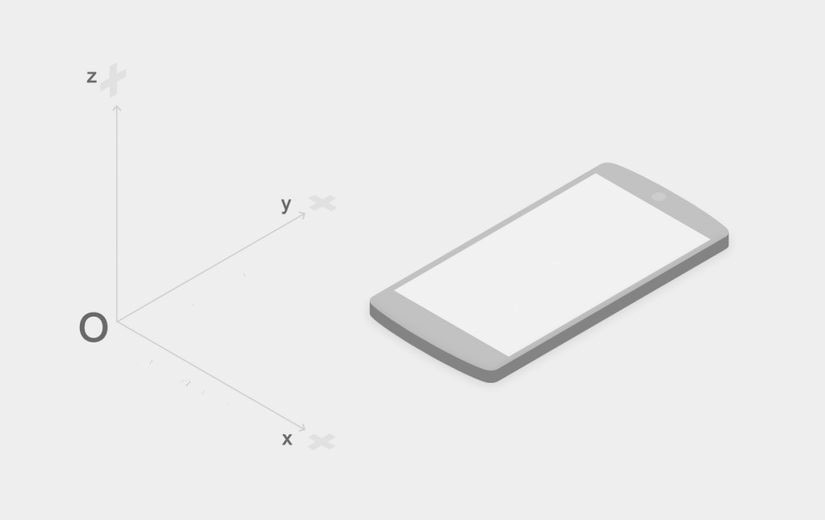
\includegraphics[width=12cm]{images/material-design-space.jpg}
% \caption{Material Design – Không gian}
% \end{figure}

% \item Thứ hai là ánh sáng:
%     Ánh sáng là yếu tố môi trường được sử dụng nhằm thể
%     hiện tính 3 chiều của không gian. Hệ quả của ánh sáng là hiệu ứng
%     đổ bóng (Drop Shadow), sẽ phân định vị trí các lớp Material trong
%     không gian theo trục Oz. Có hai loại nguồn sáng được kết hợp
%     là nguồn sáng chiếu trực tiếp và ánh sáng môi trường. Nguồn sáng
%     trực tiếp rất quan trọng, nó giống như nguồn sáng đèn pin,
%     nó mang lại hiệu ứng đổ bóng mạnh và sắc nét. Ánh sáng môi trường
%     thì nhẹ nhàng và không rõ nguồn, tạo viền bóng nhẹ xung quanh.
%     Thông thường, Material Design kết hợp cả hai nguồn sáng, mang
%     đến hiệu ứng bóng tổng hợp, mô phỏng không gian thực tế.

% \begin{figure}[H]
% \centering
% 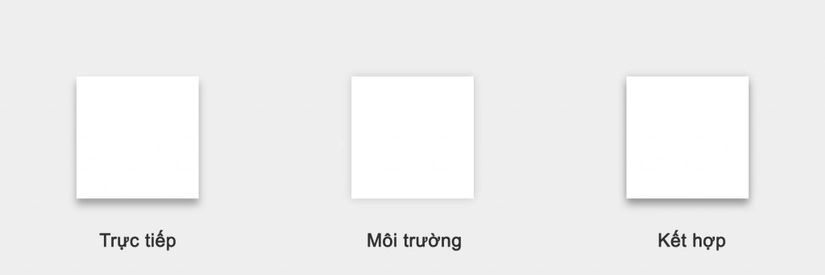
\includegraphics[width=14cm]{images/material-design-light.jpg}
% \caption{Material Design – Ánh sáng}
% \end{figure}

% \item Thứ ba là material (chất liệu): Là những mặt phẳng có độ dày
%     đồng nhất 1dp (1 in $\approx$ 160 dp) và nằm song song với mặt phẳng Oxy.
%     Các mặt phẳng Material sắp xếp chồng lên nhau theo trục Oz.
%     Thông qua việc thay đổi kích thước của bóng, ta sẽ dễ dàng
%     mô tả vị trí tương đối của mỗi lớp so với lớp khác.

% \begin{figure}[H]
% \centering
% 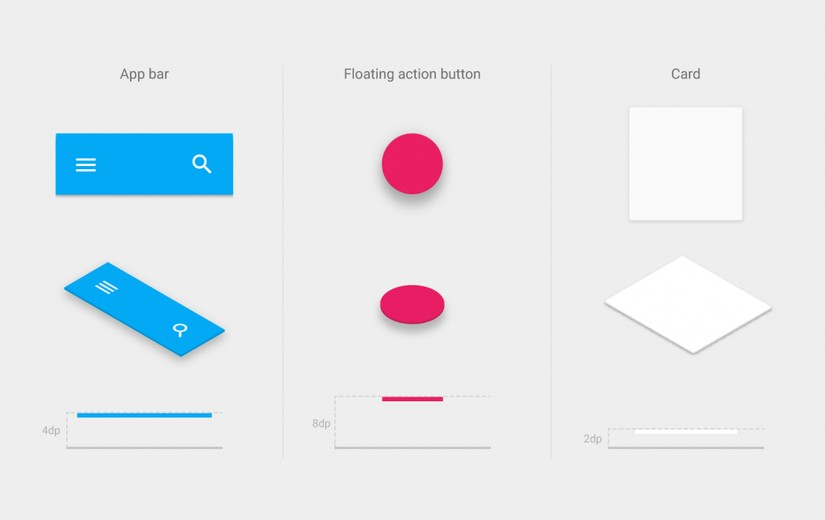
\includegraphics[width=14cm]{images/material-design-material.png}
% \caption{Material Design – Chất liệu}
% \end{figure}

% \end{itemize}

% Để có một thiết kế ấn tượng với Material Design cần
% chú ý một vài hiệu ứng và chi tiết:
% \begin{itemize}[topsep=0ex]
% \item Hiệu ứng tự nhiên: ví dụ khi bạn nhấn chọn một thành phần,
%     hiệu ứng sóng trên màn hình sẽ tỏa ra tự vị trí ngón tay
%     bạn chứ không phải từ một hướng cố định.

% \item Hiệu ứng bề mặt: khi chuyển trang, các thành phần phải chuyển
%     động một cách tự nhiên và liên tục chứ không biến mất

% \item Có thứ tự: những thành phần ở sau sẽ xuất hiện trước,
%     thành phần lớn hơn sẽ xuất hiện trước, thành phần quan trọng
%     hơn sẽ xuất hiện trước.

% \item Thống nhất: chuyển động của những Material phải thống nhất
%     từ cùng một hướng, tạo sự đồng đều cho tổng thiết kế.
% \end{itemize}

% \paragraph{Material-UI}
% Như đã trình bày ở trên, Material UI là một thư viện các
% React component tích hợp thêm Google’s Material Design.
% Material UI cung cấp khá đầy đủ các component để có thể tạo
% ra một trang web một cách nhanh chóng hơn mà không phải ngồi
% chỉnh CSS từng chút một.

% Ví dụ để tạo ra các nút bấm như hình dưới,
% ta chỉ việc sử dụng Button component mà Material UI cung cấp.
% \begin{figure}[H]
% \centering
% 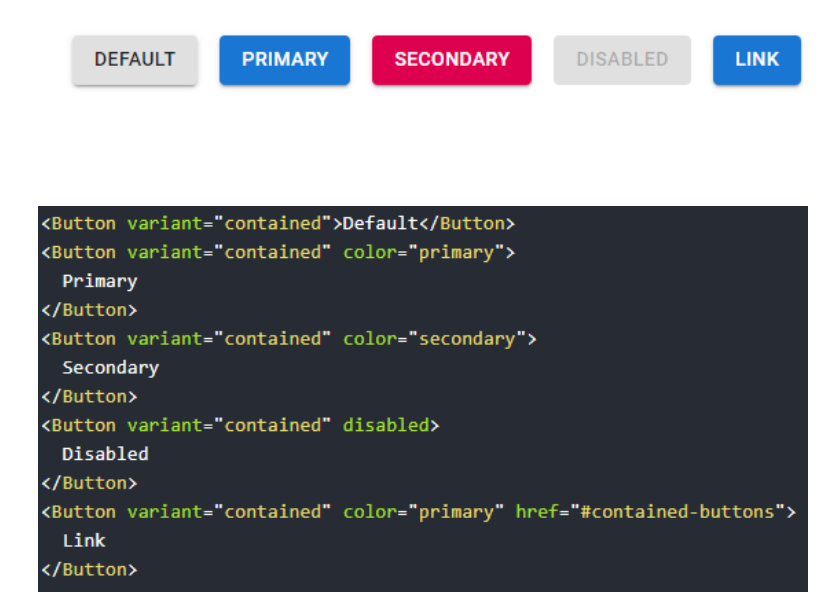
\includegraphics[width=14cm]{images/material-ui-button.png}
% \caption{Material UI – Button}
% \end{figure}

% Việc thêm màu sắc là vô cùng đơn giản với những thuộc
% tính được định nghĩa sẵn, màu sắc là chuẩn theo thiết
% kế Material Design. 
% Với Material UI, chúng ta còn dễ dàng chia bố cục và
% responsive trang web. Grid component sẽ chia màn hình theo
% bố cục 12 cột, 5 loại màn hình theo
% kích cỡ (xs, sm, md, lg, xl).

% Cùng một nội dung nhưng khi được hiển thị trên các màn
% hình khác nhau sẽ hiển thị theo cách khác nhau, đảm bảo sự thuận
% tiện nhất cho người dùng.  Thuật ngữ “Responsive Design” ám
% chỉ cách thiết kế trang web hiển thị tương thích với mọi kích thước
% thiết bị, tức là bố cục trang web sẽ tự đáp ứng theo hành vi
% người dùng và môi trường hiển thị. Môi trường này chính là kích thước
% của trình duyệt, kích thước hoặc hướng xoay thiết bị. Thiết
% kế Responsive không chỉ giúp cho người dùng có một trải nghiệm thú
% vị hơn khi truy cập website, mà còn giúp chủ sở hữu dễ dàng
% quản lý các trang web của mình hơn.

% Ngoài ra Material UI cũng có sẵn kho Icon khổng lồ trên đầy
% đủ các lĩnh vực giúp chúng ta dễ dàng chọn ra icon đẹp và
% phù hợp nhất với mỗi nội dung trên trang web.

